\chapter{Desenvolvimento do trabalho}

% Apresentar os resultados das fases que transformam
% os requisitos em produtos finais.
% • A estrutura desse capítulo depende do processo de
% desenvolvimento do trabalho.
% • A organização e as seções desse capítulo devem ser
% definidas juntamente com o orientador.

Este capítulo tem como objetivo explicitar quais foram as decisões de projeto que foram tomadas ao longo do desenvolvimento do sistema.

\section{Justificativas das métricas escolhidas}

As escolhas das métricas para o desenvolvimento desse projeto foram determinantes para avaliar e interpretar resultados com precisão. As métricas escolhidas auxiliam a avaliar o perfil dos motoristas.

\subsection{RPM}

 Em um motor de combustão interna, o RPM indica a velocidade com que os pistões se movem para cima e para baixo no cilindro. O controle preciso do RPM é essencial para otimizar a eficiência do motor e a entrega de potência, sendo um indicador chave para os motoristas ajustarem suas velocidades de condução.

 A figura \ref{fig:rpmxpotencia} mostra que a potência aumentou com o aumento da rotação do motor\textsuperscript{[28]}. Operar consistentemente em RPMs muito altos pode levar a um aumento do desgaste mecânico, já que componentes como pistões, bielas e válvulas são submetidos a forças intensas em altas velocidades. Por outro lado, operar em RPMs muito baixos pode resultar em acúmulo de resíduos e combustão incompleta, afetando negativamente a eficiência do motor.

 \begin{figure}[hp]
    \centering
    
    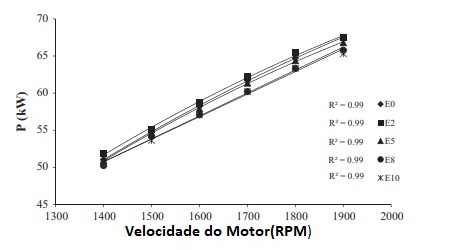
\includegraphics[scale= 1]{figures/rpmxpotencia.jpeg}
    
    \caption{Potência versus velocidade do motor.}
    
    \label{fig:rpmxpotencia}
\end{figure}

\subsection{Trajetos e rotas perigosas}

A relação entre rotas perigosas, marcadas por assaltos e roubos de carros e o perfil do motorista tornam-se elementos críticos na gestão da segurança. A escolha da rota desempenha um papel significativo na mitigação desses perigos. 

Motoristas que optam por passar frequentemente por áreas consideradas de alto risco podem estar mais suscetíveis a incidentes indesejados. Portanto, compreender o perfil do motorista em relação a essas rotas perigosas é importante para a implementação de estratégias eficazes de prevenção. 

A conscientização dos motoristas sobre áreas de risco pode contribuir para uma abordagem mais segura ao planejar e seguir rotas.
Locais como Paulista, Augusta e Sé possuem altos índices de furtos\textsuperscript{[34]}. A figura \ref{fig:mapa_risco_acc_rpm} mostra as áreas perigosas em um trajeto no bairro do Pacaembu. E as tabelas \ref{fig:tab1} e \ref{fig:tab2} mostram o tipo de risco e a fração da aceleração, respectivamente.

\begin{figure}[hp]
    \centering
    
    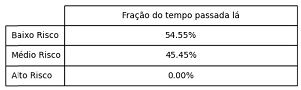
\includegraphics[scale= 1]{figures/tabela_fracao1.jpg}
    
    \caption{Potência versus velocidade do motor.}
    
    
\end{figure}

\begin{figure}[hp]
    \centering
    
    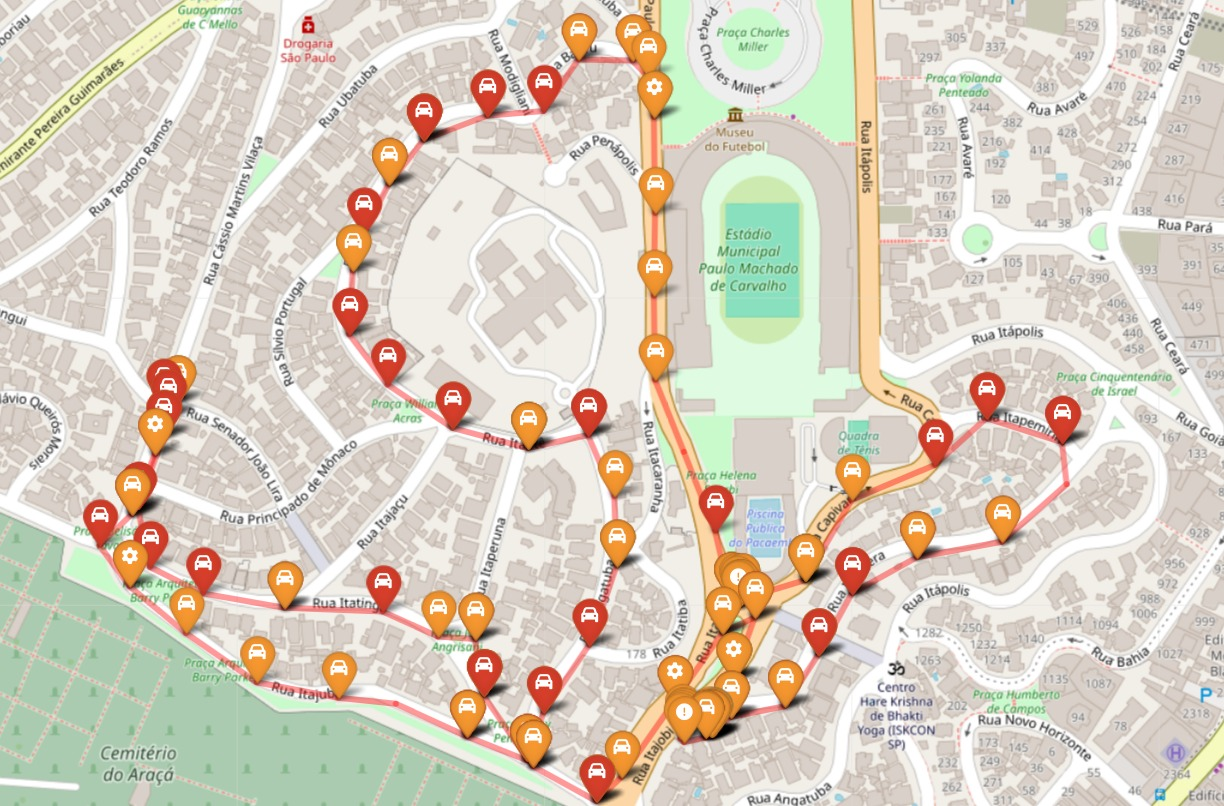
\includegraphics[scale=0.15]{figures/mapa_risco_acc_rpm.jpeg}
    
    \caption{Mapa de risco em acelerações e valor de RPM.}
    
    \label{fig:mapa_risco_acc_rpm}
\end{figure}


\begin{figure}[hp]
    \centering
    
    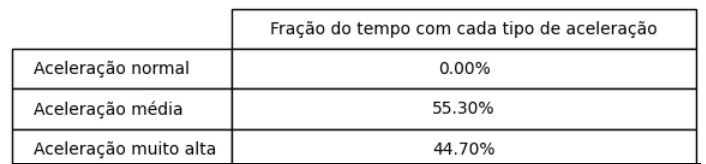
\includegraphics[scale= 0.85]{figures/tabela_2.jpg}
    
    \caption{Fração da aceleração.}
    
    \label{fig:tab1}
\end{figure}

\begin{figure}[hp]
    \centering
    
    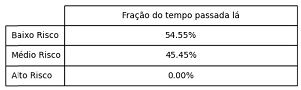
\includegraphics[scale= 0.85]{figures/tabela_fracao1.jpg}
    
    \caption{Tipo de risco.}
    
    \label{fig:tab2}
\end{figure}


A construção dessa figura foi feita graças a uma base de dados encontrada no site Kaggle\textsuperscript{[33]}, conhecido por hospedar \textit{Jupyter notebooks} analisando certos conjuntos de informações.

Embora a descrição do \textit{dataset} mencione que os dados referem-se só a São Paulo (o que já gera ambiguidade entre cidade e estado), existem lá registros de Curitiba, Rio de Janeiro e Pará também.

Importante mencionar que, devido ao tamanho dessa base de dados, de 12899 linhas, foi preciso pensar-se em como comparar os dados nela contidos com cada um dos registros de GPS fornecidos pelo \textit{app} sem que o desempenho dessa análise fosse comprometido.

Para tal, as coordenadas geográficas da planilha foram indexadas da seguinte forma: 

\begin{python}
def convert_coord_to_chunk(self, coord_1, coord_2, max_coord_diff):
    coord_diff = coord_1 - coord_2
    chunk = (self.segmentation_rate * coord_diff) // max_coord_diff
    return chunk

    self.north = car_crimes_df["latitude"].max() + (0.5 / 111.11)
    self.south = car_crimes_df["latitude"].min() - (0.5 / 111.11)
    self.west = car_crimes_df["longitude"].max() + (0.5 / 111.11)
    self.east = car_crimes_df["longitude"].min() - (0.5 / 111.11)

    # maior distancia de norte a sul: 4378.4 km
    # maior distancia de leste a oeste: 4326.6 km
    self.segmentation_rate = 4400

    self.lat_diff = self.north - self.south
    self.long_diff = self.east - self.west

    
    car_crimes_df["chunk_i"] = car_crimes_df["latitude"]
        .apply(lambda x : 
        self.convert_coord_to_chunk(x, self.south, self.lat_diff))
    car_crimes_df["chunk_j"] = car_crimes_df["longitude"]
        .apply(lambda x : 
        self.convert_coord_to_chunk(x, self.west, self.long_diff))
\end{python}

Alguns números mágicos utilizados levaram em consideração a equivalência entre graus e quilômetros da Terra e as distâncias entre os pontos mais a sul, norte, leste e oeste do Brasil\textsuperscript{[35, 36]}.

A ideia dessa indexação é dividir o mapa em \textit{chunks}, os quais limitam o trabalho computacional a um subconjunto dos dados. Cada \textit{chunk} é um quadrado de lado 500m, o que obriga o programa a olhar alguns blocos adjacentes ao onde está a coordenada cuja segurança quer-se verificar.

% \begin{figure}[hp]
%     \centering
    
%     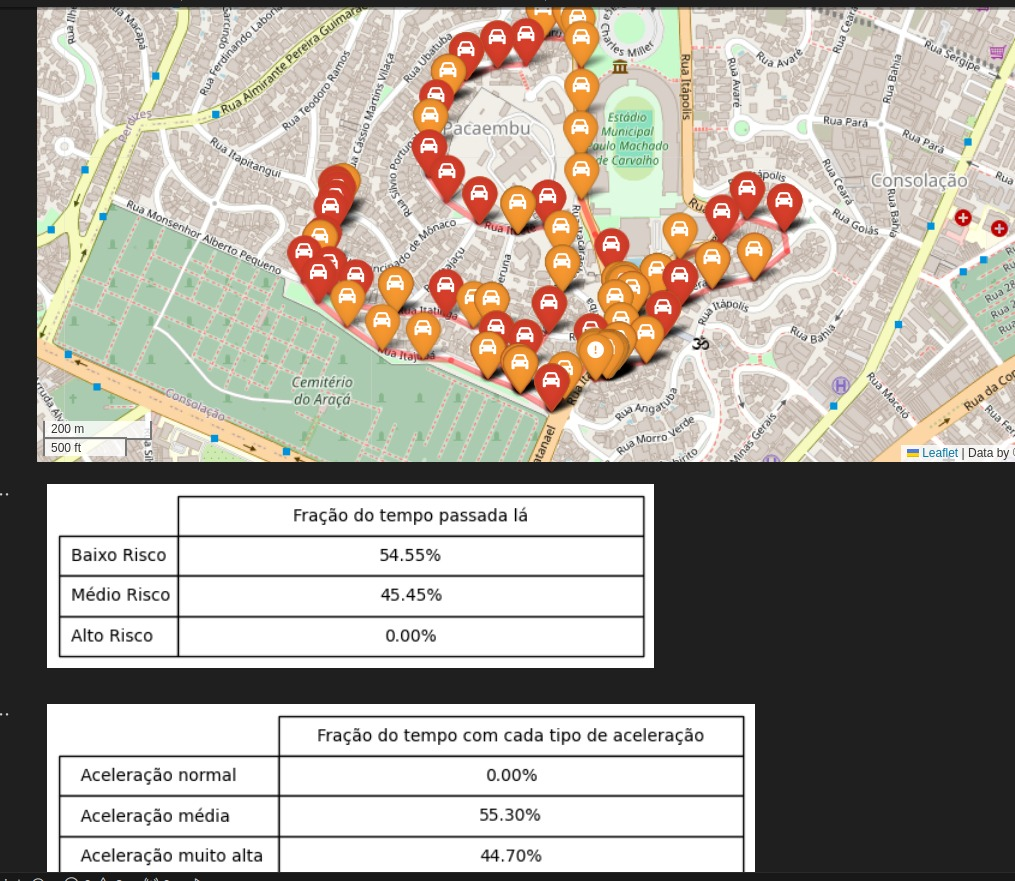
\includegraphics[scale=0.8]{figures/rotas_altorisco.jpeg}
    
%     \caption{}
    
%     \label{fig:rotas_altorisco}
% \end{figure}

 
\section{Tecnologias utilizadas}
O projeto pretende definir algumas tecnologias de base para serem usadas durante o desenvolvimento de cada fase dele.

    \subsection{Amazon Web Services}

    A escolha da AWS para o projeto é fundamentada em três pilares essenciais: escalabilidade, segurança e viabilidade econômica. 
    
    A capacidade desse serviço de nuvem de se adaptar dinamicamente às demandas do sistema assegura uma infraestrutura flexível, capaz de lidar eficientemente com variações na carga de trabalho. 
    
    Além disso, a reputação consolidada da Amazon em termos de segurança oferece uma base robusta para proteção dos dados e operações. 
    
    Por fim, a viabilidade econômica se destaca, uma vez que a AWS disponibiliza uma variedade de serviços e modelos de precificação que se alinham de maneira eficaz às necessidades do projeto, otimizando custos operacionais.

    É evidente que todas essas vantagens só são concretizadas caso os implementadores do sistema façam uso de toda a funcionalidade da nuvem: projetos monolíticos, ainda que rodados em servidores distribuídos, não exploram a flexibilidade de serviços como a AWS. 

    \subsection{Conexão OBD-II}

    A integração do OBD-II (\textit{On-Board Diagnostics}) neste projeto de sistema de coleta de dados representa um avanço significativo na obtenção de dados precisos e abrangentes sobre o desempenho do veículo. O OBD-II, um padrão presente em muitos veículos modernos, fornece acesso a uma variedade de parâmetros, como velocidade, rotações por minuto (RPM), temperatura do motor, e códigos de diagnóstico de falhas. Ao conectar a plataforma de captura de dados ao conector OBD-II do veículo, é possível extrair informações em tempo real sobre a condução, condições do motor e possíveis problemas mecânicos.

    Já existe uma plataforma aceleradora desenvolvida no GitHub que consegue comunicar-se com o veículo através do protocolo OBD-II\textsuperscript{[12]}. 
    
    Esse outro projeto implementa o protocolo OBD-II e também uma interface gráfica básica para mostrar os dados fornecidos pelo carro.

    A figura \ref{fig:obd2_plataforma} mostra uma plataforma onde é possível ver alguns dos dados quando o motorista estava dando uma volta ao redor do bairro.

\begin{figure}[hp]
    \centering
    
    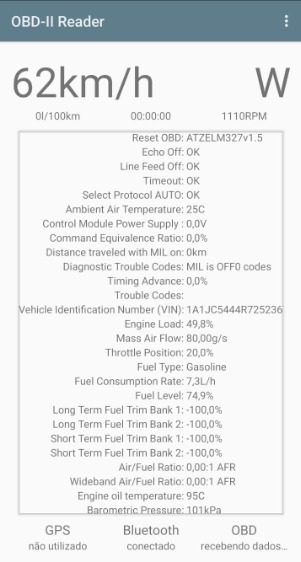
\includegraphics[scale=0.5]{figures/obd2.jpeg}
    
    \caption{Interface básica com porta OBD-II\textsuperscript{[12]}.}
    
    \label{fig:obd2_plataforma}
\end{figure}
    
    \subsection{Android Studio} A utilização da IDE Android Studio neste projeto de sistema de coleta de dados desempenha um papel central no desenvolvimento de aplicativos móveis dedicados à interação com o sistema. 
    
    O Android Studio, sendo a principal ferramenta de desenvolvimento para aplicativos Android, oferece um ambiente integrado e robusto que simplifica a criação, teste e depuração de software. 
    
    A plataforma fornece recursos avançados de design de interface do usuário, facilitando a criação de aplicativos intuitivos e visualmente atraentes para os usuários finais. A integração perfeita com o Android SDK (Software Development Kit) permite o acesso às APIs e recursos específicos do sistema operacional Android, garantindo uma implementação eficiente de funcionalidades como a transmissão Bluetooth, a visualização de dados de rastreamento e a interação em tempo real. 
    
    Além disso, as ferramentas de emulação e depuração incorporadas no Android Studio simplificam o processo de teste em diferentes dispositivos, contribuindo para a criação de aplicativos estáveis e adaptáveis.

    Por último, nenhuma tecnologia multiplataforma (React Native ou Flutter, por exemplo) ou específica de dispositivos iOS (Swift ou Objective C, por exemplo) foi escolhida, pois o intuito do projeto era ser compatível com os celulares dos membros do grupo e devido à familiaridade com a linguagem Java, usada para esse tipo de desenvolvimento.

    O aplicativo em si (arquivo SDK) originalmente foi desenvolvido para a API de versão 22 do Android

     \begin{figure}[hp]
    \centering
    
    
\includegraphics[scale=0.4]{figures/logo_android.png}
    
    \caption{Logo Android Studio.}
    
\end{figure}
    
     \subsection{Banco de dados} A integração do MySQL e do AWS RDS (Relational Database Service) em um projeto de sistema de compilação de dados de veículos é uma estratégia robusta para o gerenciamento eficiente e escalável dos dados do sistema. O MySQL, um sistema de gerenciamento de banco de dados relacional de código aberto, proporciona uma estrutura confiável para armazenar e organizar informações como histórico de rotas e dados do OBD-II. 
     
     Ao escolher o AWS RDS como a plataforma de hospedagem para o MySQL, ganha-se os benefícios adicionais de escalabilidade automática, alta disponibilidade e segurança avançada oferecidos pela infraestrutura em nuvem da Amazon. A integração dessas tecnologias permite o acesso eficiente aos dados, consultas rápidas e uma gestão simplificada do banco de dados. 
     
     Além disso, o AWS RDS lida com tarefas operacionais, como backup automático e manutenção, permitindo que os desenvolvedores concentrem seus esforços em aprimorar as funcionalidades do sistema de rastreamento. 
     
     Essa combinação proporciona uma base sólida para o armazenamento e recuperação de dados, promovendo a confiabilidade e eficácia do sistema.

     A estrutura definida para as tabelas do banco de dados foi:


    \begin{itemize}
         \item{\textbf{tcc-schema} (esquema do banco de dados onde se encontram as tabelas)}
         
        \begin{itemize}
             \item{\textbf{info:} Armazena as informações coletadas através da porta OBD} 
        
             \item{\textbf{acceleration:} Contém dados dos acelerômetros do celular do usuário} 
             
             \item{\textbf{location:} Guarda latitude e longitude obtidas por GPS pelo celular}   
        \end{itemize}  
    \end{itemize}

     A especificação exata das colunas de cada tabela pode ser encontrada no apêndice. [MENCIONAR APENDICE POR NUMERO]

    \begin{figure}[hp]
        \centering
        
        
\includegraphics[scale=0.4]{figures/logo_Mysql.jpg}
        
        \caption{Logo do Mysql.}
        
    \end{figure}

    
     \subsection{\textit{Python} e Folium} A junção do Python e do Folium em um projeto de sistema de coleta de dados oferece uma poderosa combinação para a visualização interativa e geoespacial dos dados. O Folium é uma biblioteca Python que simplifica a criação de mapas interativos baseados na web, utilizando a infraestrutura do Leaflet.js. Integrar o Folium ao projeto permite que os desenvolvedores gerem mapas dinâmicos que destacam informações específicas relacionadas ao rastreamento de veículos.

    Essa integração Python-Folium é particularmente útil para análises geoespaciais em sistemas de rastreamento de veículos, proporcionando uma representação geográfica e visualmente intuitiva dos dados de telemetria. 
    
    A flexibilidade do Python permite a personalização dos mapas e a incorporação de recursos adicionais conforme as necessidades específicas do projeto, contribuindo para uma interface de usuário mais informativa e envolvente.

      \begin{figure}[hp]
    \centering
    
    
\includegraphics[scale=0.1]{figures/python_folium.jpg}
    
    \caption{Logo Python + Folium.}
\end{figure}

% interface com usuario, banco de dados, conexão obd2

    \subsection{Flask}

    A seleção da biblioteca Flask para o projeto ocorreu devido à familiaridade com a linguagem Python, tornando o desenvolvimento mais acessível. Adicionalmente, a escolha se fundamentou na capacidade do Flask em facilitar a implementação eficiente de uma API, atendendo à necessidade do aplicativo de enviar e receber dados de maneira eficaz. O código python da API em Flask foi hospedado em um Lambda da AWS para facilitar o seu uso pelo APP posteriormente.


\section{Projeto e implementação}
% Esta seção descreverá as decisões feitas durante o trabalho.

\subsection{Folium}
    Para criar os mapas do aplicativo, foi utilizado o \textit{framework} Folium. Essa biblioteca é uma poderosa ferramenta para manipular e visualizar dados geoespaciais usando Python. 
    
    Com o Folium, é possível criar mapas interativos personalizados e incorporar dados neles de várias maneiras. Para manipular dados usando essa ferramenta, pode-se começar importando a biblioteca e criando um objeto Map que representa o mapa. 
    
    Em seguida, pode-se adicionar camadas, como marcadores, polígonos e \textit{popups}, para exibir dados de forma intuitiva no mapa. 
    
    % O Folium permite a integração de dados geoespaciais em diferentes formatos, como GeoJSON, tornando-o uma ferramenta flexível para análise e visualização de dados geoespaciais em Python. 
    
    A figura 
    \ref{fig:python_libs} mostra as bibliotecas utilizadas para desenvolver os mapas do projeto.
    
    \begin{figure}[hp]
        \centering
        
        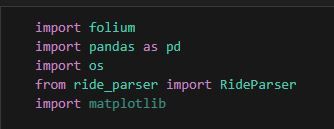
\includegraphics[scale=0.8]{figures/bibliotecas.jpg}
        
        \caption{Bibliotecas utilizadas para gerar o mapa da rota do usuário.}
        
        \label{fig:python_libs}
    \end{figure}
    
            % \begin{center}
            %  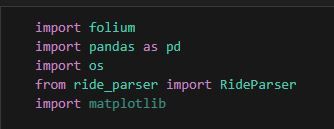
\includegraphics[scale=0.8]{figures/bibliotecas.jpg}
            %  
            %  \end{center}
            
    Para traçar uma trajetória no mapa usando a biblioteca Folium em Python, será necessário uma lista de pontos de latitude e longitude que representam a trajetória. A partir dos pontos de latitude e longitude colhidos dos sensores do celular, cria-se uma lista de coordenadas que representam os pontos da trajetória. Em seguida, criamos um objeto de mapa usando o Folium e é adicionado uma linha de trajetória (um polilinha) que conecta os pontos da lista e o mapa pode ser visualizado. Uma demonstração de uma trajetória pode ser vista na figura \ref{fig:car_route_1}.
    
    \begin{figure}[hp]
        \centering
        
        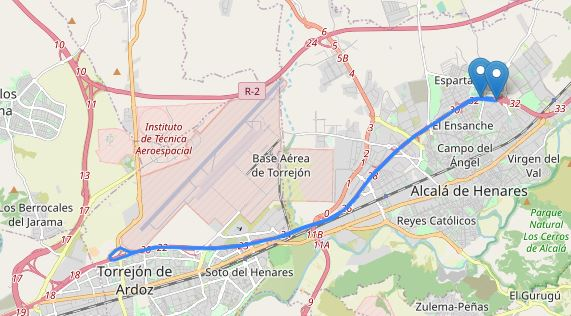
\includegraphics[scale=0.8]{figures/rota_1.jpg}
        
        \caption{Rota de uma das viagens fornecidas pelo \textit{UAH Driveset}.}
        
        \label{fig:car_route_1}
    \end{figure}
    
    A visualização de um vídeo que apresenta o trajeto do veículo sincronizado com um gráfico de aceleração proporciona uma compreensão visual e analítica aprimorada do comportamento de condução. Este recurso permite aos usuários acompanhar de forma imersiva o percurso do veículo enquanto simultaneamente observam as variações na aceleração ao longo do tempo. 
    
    Ao visualizar o vídeo, os usuários podem identificar eventos específicos, como curvas acentuadas, frenagens bruscas ou acelerações rápidas, correlacionando-os diretamente com os picos e quedas no gráfico de aceleração exibido ao lado. Essa abordagem oferece uma representação mais holística da experiência de condução, permitindo uma análise detalhada de como o estilo de direção afeta diretamente a aceleração do veículo. 
    
    Além disso, essa visualização combinada pode ser uma ferramenta valiosa para treinamento de motoristas, análise de incidentes e \textit{feedbacks} personalizados, proporcionando uma compreensão mais rica e envolvente do desempenho do veículo e do comportamento do condutor.

    \subsection{Análise de Dados - RideParser}\label{rideparser}

    A função da classe RideParser é analisar dados dos trajetos feitos pelos motoristas. 
    
    Alguns filtros são recebidos pelo construtor dessa classe, para personalizar a geração de gráficos. Esses parâmetros são usados para restringir o que vem do banco de dados a uma certa janela de tempo e ao usuário que solicita aquela informação.
    
    % Já o módulo 
    % ''os'' fornece funcionalidades relacionadas ao sistema operacional, permitindo que você interaja com o ambiente do sistema, como manipular diretórios, arquivos, obter informações sobre o sistema, manipular variáveis de ambiente, entre outras tarefas relacionadas ao sistema operacional.
    Dentro desse mesmo arquivo, algumas bibliotecas típicas de ciência de dados foram utilizadas para manipular os gráficos mencionados. Foram elas: pandas, matplotlib, numpy e scipy.
    
    A figura \ref{fig:rota1integrante} mostra o video e o gráfico da aceleração.
    
    \begin{figure}[hp]
        \centering
        
        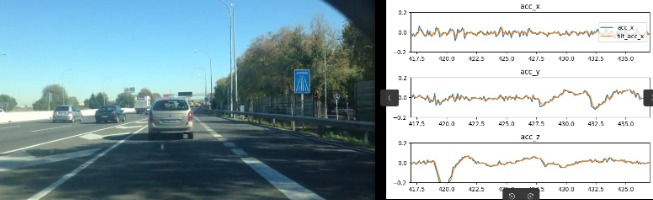
\includegraphics[scale=0.6]{figures/rota_integrante.jpg}
        
        \caption{Rota de uma viagem de um dos integrantes do grupo.}
        \label{fig:rota1integrante}
    \end{figure}

    \subsection{API Rest - Flask}
    A implementação da API centraliza-se em uma arquitetura Python utilizando a biblioteca Flask, proporcionando uma estrutura ágil e eficiente para a comunicação com a base de dados MySQL, hospedada em um serviço de RDS na AWS. A escolha da linguagem Python e do framework Flask foi motivada pela sua simplicidade e flexibilidade, permitindo a rápida construção dos endpoints responsáveis pela interação entre o aplicativo e a base de dados.

    A lógica da API foi encapsulada em funções específicas, acionadas por meio de requisições POST. O corpo do JSON enviado nessas requisições determina a ação a ser executada, que pode ser uma entre seis operações distintas. Três destas operações referem-se a consultas (GET) e três a modificações (POST), cada uma vinculada a uma das três tabelas da base de dados.

    Para facilitar a utilização da API pelo app, o código Python foi integrado ao ambiente serverless da AWS Lambda. Essa escolha estratégica permite que as funções sejam invocadas sob demanda, proporcionando uma resposta ágil às requisições do aplicativo Android, que, por sua vez, está sendo desenvolvido no ambiente Java do Android Studio. A combinação dessas tecnologias promove uma arquitetura eficiente para gerenciar a comunicação entre o aplicativo e a infraestrutura de banco de dados na nuvem.


    \subsection{Criação de relatório em PDF}
    
    A geração de insights visuais e análise métrica a partir dos dados armazenados na base MySQL é um componente essencial do projeto. A decisão de fazer isso através da geração de um PDF para o motorista baseou-se na clareza e simplicidade desse formato de arquivo. Essa escolha é respaldada também pela facilidade de implementação, disponibilizada pela biblioteca \textit{Matplotlib}, que permite a criação de PDFs formatados contendo os gráficos com as métricas geradas.
    
    Um segundo AWS Lambda desempenha um papel central nesse processo, funcionando como uma ponte entre a base de dados e as ferramentas de visualização. Ao ser acionado, esse Lambda realiza uma chamada ao outro Lambda, que extrai as informações relevantes da base de dados MySQL referentes ao usuário, para realizar a análise.

    Utilizando a biblioteca Matplotlib em Python, a função Lambda então emprega métodos da classe RideParser, mencionada na sessão \ref{rideparser}, para criar um relatório do motorista, com gráficos e métricas relevantes referentes a sua condução. Isso proporciona aos usuários uma compreensão mais aprofundada das métricas associadas às suas atividades.
    
    Para proporcionar aos usuários uma maneira acessível de interagir com esses insights, um botão "gerar PDF" foi incorporado no aplicativo. Este botão aciona o segundo Lambda, que compila os gráficos e métricas gerados em um arquivo PDF. A utilização da biblioteca smtplib facilita o envio desse PDF diretamente para o usuário via email. Essa solução integrada oferece uma experiência completa aos usuários, permitindo-lhes não apenas visualizar, mas também compartilhar os resultados de suas análises de maneira eficaz.    

    \subsection{Autenticação com \textit{Firebase}}

    A  escolha do \textit{Firebase} para a identificação única do usuário no sistema decorre da capacidade da plataforma em oferecer eficiência e segurança nesse processo, diminuindo-se a carga de responsabilidade do sistema em armazenar informações sensíveis de cada pessoa. 
    
    Essa decisão é fundamentada pela praticidade proporcionada pela integração do \textit{Firebase} com aplicativos \textit{Android} e páginas web\textsuperscript{[29]}, simplificando a implementação de autenticação e gestão de usuários, assegurando uma identificação singular e segura no âmbito do sistema em questão.

    \subsection{Dependências do Gradlle}

    Em um primeiro instante o app android-obd-reader não queria rodar na IDE Android studio. Para que isso fosse possível foi necessario fazer alterações no arquivo \textbf{gradle/wrapper/gradle-wrapper.properties}. Atualizar as dependências do Gradle  é muitas vezes necessário para garantir que o seu aplicativo possa se beneficiar das correções de bugs, melhorias de desempenho e novos recursos fornecidos pelas versões mais recentes das bibliotecas que você está utilizando. Este link \url{https://github.com/APF2000/android-obd-reader-pires/commit/def70ed262b1fad28cc9e2b98a48af45cfac5695} mostra as alterações que foram necessárias.

    \subsection{Proteção dos dados}
    
    Na Lei Geral de Proteção de Dados (Lei n. 13.709/18-LGPD), parte-se da ideia de que todo dado pessoal tem importância e valor. Por essa razão se adotou conceito amplo de dado pessoal, assim como estabelecido no Regulamento europeu \textsuperscript{[30]} (GDPR-General Data Protection  Regulation). Quando se trata de um aplicativo projetado para analisar o perfil do motorista de carros, a LGPD impõe uma série de responsabilidades e requisitos ao desenvolvedor e operador do aplicativo. É necessário obter o consentimento  do usuário antes de coletar e processar quaisquer dados pessoais relacionados ao seu perfil de condução.
    
    Além disso, a LGPD exige que medidas de segurança apropriadas sejam implementadas para proteger esses dados contra acessos não autorizados e vazamentos. Os usuários têm o direito de acessar, corrigir e excluir suas informações pessoais, e o aplicativo deve fornecer meios para que esses direitos sejam exercidos.


% Using \texttt{biblatex} you can display a bibliography divided into sections, depending on citation type. 
% Let's cite! Einstein's journal paper \cite{einstein} and Dirac's book \cite{dirac} are physics-related items. 
% Next, \textit{The \LaTeX\ Companion} book \cite{latexcompanion}, Donald Knuth's website \cite{knuthwebsite}, \textit{The Comprehensive Tex Archive Network} (CTAN) \cite{ctan} are \LaTeX-related items; but the others, Donald Knuth's items, \cite{knuth-fa,knuth-acp} are dedicated to programming. 




\section{Testes e avaliação}
% descrever o plano de testes do sistema: testes de software, modulo, integração e validação
Alguns testes foram definidos para a ratificação das funcionalidades do sistema:

\begin{itemize}
    \item \textbf{Conferir conexão OBD-II:} 
    
    \begin{itemize}
        \item Conectar o dispositivo de leitura na entrada do carro
        \item Ligar a comunicação \textit{bluetooth} do celular
        \item Parear os dois dispositivos
        \item Digitar a senha 1234, padrão dos dispositivos de leitura OBD
        \item Ligar a coleta de dados através do aplicativo
        \item A tela deve sinalizar que o protocolo está sendo feito da forma correta
    \end{itemize}
    
    \item \textbf{Teste de continuidade de transferência de dados:} 
    \begin{itemize}
        \item Fazer conexão com o OBD conforme descrito no teste anterior
        \item Andar com o carro por alguns minutos com a tela do celular desbloqueada (de preferência mudar o \textit{timeout} da tela nas configuraçõs do celular)
        \item Atestar que nenhum dado foi perdido por falta de conexão (pode ser visto por descontinuidade dos gráficos)
    \end{itemize}
    
    \item \textbf{Equivalência de envio e recepção de dados:}
    \begin{itemize}
        \item Comparar o \textit{log} de envio de dados do aplicativo de interface com a porta OBD-II com o \textit{log} de salvamento do banco de dados hospedado na nuvem
        \item A quantidade de dados, os \textit{timestamps} deles e seus conteúdos devem ser idênticos
    \end{itemize}
    
    \item \textbf{Testes de segurança:} 
    \begin{itemize}
        \item Ratificar que não é possível ter acesso aos dados de um certo usuário sem ter as informações de \textit{login}
        \item Verificar o certificado SSL do remetente e só aceitar a mensagem se a informação condisser com as credenciais armazenadas daquele usuário
    \end{itemize}
    
    \item \textbf{Geração de dados \textit{outliers}:}
    \begin{itemize}
        \item Verificar se o sistema descarta corretamente as informações que fogem totalmente do padrão esperado ou se consegue pelo menos esconder isso do usuário
        \item Os PDFs gerados com o sistema devem sofrer um processo de análise de plausibilidade, o que deve averiguar que a análise automática está sendo feita corretamente
    \end{itemize}
    
\end{itemize}


\subsection{Fluxo de uso do sistema}

    \begin{itemize}
    \item \textbf{Autenticação com o Google:}
    O aplicativo no celular deve ser iniciado para realizar a autenticação com as credenciais do Google, assegurando uma identificação segura do usuário.

    \item \textbf{Conexão com o OBD:}
    A conexão entre o celular e o OBD deve ser estabelecida, garantindo que o leitor esteja corretamente emparelhado para iniciar a comunicação.

    \item \textbf{Início da Coleta de Dados:}
    A coleta de dados deve ser ativada por meio do aplicativo.

    \item \textbf{Condução do Veículo:}
    O veículo deve ser conduzido normalmente, permitindo que o aplicativo faça a coleta de dados em tempo real.

    \item \textbf{Posicionamento Fixo do Celular:}
    O celular deve ser fixado em uma posição estável dentro do veículo usando um suporte apropriado. Isso garantirá que os dados de aceleração sejam confiáveis, o que evitará qualquer tipo de interferência na análise posterior da direção.
\end{itemize}


\subsection{Carros utilizados para teste}

    A escolha dos carros onde o leitor de OBD seria conectado foi feita a partir dos veículos de familiares.

    Os modelos em que o sistema foi testado, foram em maioria para analisar quais parâmetros de OBD haviam sido implementados em todos eles.

    Os carros usados foram:

    \begin{itemize}
        \item Hyundai Ix35 - 2012
        \item Mercedes C200 CGI - 2014
        \item Ford Xsport - 2008
    \end{itemize}

    

    O modelo Ix35 foi a principal fonte de dados do projeto, pois praticamente todos os testes feitos para a nova base de dados foram feitos com ele.

    \subsection{Aparelhos \textit{smartphone}}

    O aplicativo foi rodado em dois modelos diferentes de celular:
    \begin{itemize}
        \item Samsung Galaxy A71
        \item Samsung Galaxy S9
        \item Samsung Galaxy S22
        \item Motorola Moto G
    \end{itemize}

\subsection{Definição de dados relevantes para o perfilamento}

    Os parâmetros identificados em comum em todos os carros testados foram: \textit{AIR-FUEL-RATIO, AIR-INTAKE-TEMP, AMBIENT-AIR-TEMP, BAROMETRIC-PRESSURE, CONTROL-MODULE-VOLTAGE, DISTANCE-TRAVELED-MIL-ON, DTC-NUMBER, ENGINE-COOLANT-TEMP, ENGINE-LOAD, ENGINE-OIL-TEMP, ENGINE-RPM, ENGINE-RUNTIME, EQUIV-RATIO, Echo Off, FUEL-CONSUMPTION-RATE, FUEL-LEVEL, FUEL-PRESSURE, FUEL-RAIL-PRESSURE, FUEL-TYPE, INTAKE-MANIFOLD-PRESSURE, Line Feed Off, Long Term Fuel Trim Bank 1, Long Term Fuel Trim Bank 2, MAF, Reset OBD, SPEED, Select Protocol AUTO, Short Term Fuel Trim Bank 1, Short Term Fuel Trim Bank 2, THROTTLE-POS, TIMING-ADVANCE, TROUBLE-CODES, Timeout, VIN, WIDEBAND-AIR-FUEL-RATIO}.

    No entanto, muitas dentre essas informações ou apresentavam o valor \textit{NODATA}, que significa que estavam sendo amostrados pelo OBD, mas não continham dados válidos, ou apresentavam dados constantes, os quais independem da direção do motorista.

    Os \textbf{parâmetros descartados} foram \textit{CONTROL-MODULE-VOLTAGE, DISTANCE-TRAVELED-MIL-ON, DTC-NUMBER, Echo Off, ENGINE-OIL-TEMP, FUEL-CONSUMPTION-RATE, FUEL-LEVEL, FUEL-PRESSURE, FUEL-RAIL-PRESSURE, FUEL-TYPE, Line Feed Off, Long Term Fuel Trim Bank 2, MAF, Reset OBD, Select Protocol AUTO, Short Term Fuel Trim Bank 2, Timeout, TROUBLE-CODES, VIN, WIDEBAND-AIR-FUEL-RATIO}.
    
    Os \textbf{parâmetros considerados} para uso foram \textit{AIR-FUEL-RATIO, AIR-INTAKE-TEMP, AMBIENT-AIR-TEMP, BAROMETRIC-PRESSURE, ENGINE-COOLANT-TEMP, ENGINE-LOAD, ENGINE-RPM, ENGINE-RUNTIME, EQUIV-RATIO, INTAKE-MANIFOLD-PRESSURE, Long Term Fuel Trim Bank 1, Short Term Fuel Trim Bank 1, SPEED, THROTTLE-POS, TIMING-ADVANCE}.
    
    Entre os dados candidatos para serem usados no projeto, apenas os que foram \textbf{citados em artigos científicos} como determinantes para o acontecimento de acidentes e a deterioração do carro foram de fato levados em consideração: \textit{ENGINE-RPM}\textsuperscript{[28]}, \textit{SPEED}\textsuperscript{[32]}

            %     \item CONTROL-MODULE-VOLTAGE
            % \item DISTANCE-TRAVELED-MIL-ON
            % \item DTC-NUMBER
            % \item Echo Off
            % \item ENGINE-OIL-TEMP
            % \item FUEL-CONSUMPTION-RATE
            % \item FUEL-LEVEL
            % \item FUEL-PRESSURE
            % \item FUEL-RAIL-PRESSURE
            % \item FUEL-TYPE
            % \item Line Feed Off
            % \item Long Term Fuel Trim Bank 2
            % \item MAF
            % \item Reset OBD
            % \item Select Protocol AUTO
            % \item Short Term Fuel Trim Bank 2
            % \item Timeout
            % \item TROUBLE-CODES
            % \item VIN
            % \item WIDEBAND-AIR-FUEL-RATIO

            % \item AIR-FUEL-RATIO
            % \item AIR-INTAKE-TEMP
            % \item AMBIENT-AIR-TEMP
            % \item BAROMETRIC-PRESSURE
            % \item ENGINE-COOLANT-TEMP
            % \item ENGINE-LOAD
            % \item ENGINE-RPM
            % \item ENGINE-RUNTIME
            % \item EQUIV-RATIO
            % \item INTAKE-MANIFOLD-PRESSURE
            % \item Long Term Fuel Trim Bank 1
            % \item Short Term Fuel Trim Bank 1
            % \item SPEED
            % \item THROTTLE-POS
            % \item TIMING-ADVANCE


    % \begin{itemize}
    %     \item AIR-FUEL-RATIO
    %     \item AIR-INTAKE-TEMP
    %     \item AMBIENT-AIR-TEMP
    %     \item BAROMETRIC-PRESSURE
    %     \item CONTROL-MODULE-VOLTAGE
    %     \item DISTANCE-TRAVELED-MIL-ON
    %     \item DTC-NUMBER
    %     \item ENGINE-COOLANT-TEMP
    %     \item ENGINE-LOAD
    %     \item ENGINE-OIL-TEMP
    %     \item ENGINE-RPM
    %     \item ENGINE-RUNTIME
    %     \item EQUIV-RATIO
    %     \item Echo Off
    %     \item FUEL-CONSUMPTION-RATE
    %     \item FUEL-LEVEL
    %     \item FUEL-PRESSURE
    %     \item FUEL-RAIL-PRESSURE
    %     \item FUEL-TYPE
    %     \item INTAKE-MANIFOLD-PRESSURE
    %     \item Line Feed Off
    %     \item Long Term Fuel Trim Bank 1
    %     \item Long Term Fuel Trim Bank 2
    %     \item MAF
    %     \item Reset OBD
    %     \item SPEED
    %     \item Select Protocol AUTO
    %     \item Short Term Fuel Trim Bank 1
    %     \item Short Term Fuel Trim Bank 2
    %     \item THROTTLE-POS
    %     \item TIMING-ADVANCE
    %     \item TROUBLE-CODES
    %     \item Timeout
    %     \item VIN
    %     \item WIDEBAND-AIR-FUEL-RATIO
    % \end{itemize}